\documentclass[a4paper, 12pt]{article}
\usepackage[a4paper, left=0.4cm, right=0.4cm, top=0.4cm, bottom=0.4cm, landscape]{geometry}
\usepackage{multicol}
\usepackage{listings}
\usepackage{enumitem}
\usepackage{graphicx}
\usepackage{courier}
\usepackage{vwcol}
\usepackage{amsmath}
\usepackage{amssymb}

\setitemize{noitemsep,topsep=0pt,parsep=0pt,partopsep=0pt,leftmargin=*}
\setenumerate{noitemsep,topsep=0pt,parsep=0pt,partopsep=0pt,leftmargin=*}
\lstset{
	belowskip=0.1em,
	aboveskip=0.1em,
	basicstyle=\ttfamily,
}

\begin{document}
\setlength\parindent{0pt}
\scriptsize
\pagenumbering{gobble}

\begin{center}
{\normalsize\textbf{ST2334 Cheatsheet 19/20 S1 Midterms}}
\end{center}
\begin{multicols*}{3}
\noindent
{\small\textbf{Definitions}}
\begin{itemize}
    \item Sample Space: $S$ is the set of all possible outcomes
    \begin{itemize}
        \item eg. For rolling 2 dice: $S = \{(1,1),(1,2)...(6,5),(6,6)\}$
    \end{itemize}
    \item Sample Point: Any element/outcome in the sample space $S$
    \item Event: Any subset $E$ of the sample space
    \item Sure Event: the sample space itself
    \item Null Event: empty set $\emptyset$
\end{itemize}

\medskip
{\small\textbf{Counting}} \\
\begin{tabular}{ |c|c c| } 
\hline
Choose $k$ from $n$ & Order Matters & Not Matter \\ 
\hline
With Replacement & $n^k$ & $\binom{n + k - 1}{k}$\\ 
Without Replacement & $\frac{n!}{(n - k)!}$ & $\binom{n}{k}$ \\ 
\hline
\end{tabular}
\begin{itemize}
    \item In a circle: $(n - 1)!$ 
\end{itemize}
\medskip

{\small\textbf{Probability}} \\
\textbf{Inclusion-Exclusion Principle}
\begin{itemize}
    \item $P(A \cup B) = P(A) + P(B) - P(A \cap B)$
    \item $P(A \cup B \cup C) = P(A) + P(B) + P(C)$
    $- [P(A \cap B) + P(A \cap C) + P(B \cap C)]$ \\
    $+ P(A \cap B \cap C)$
\end{itemize}
\textbf{Independent Events}
\begin{itemize}
    \item $P(A \cap B) = P(A) \times P(B)$
    \item $P(A|B) = P(A)$
    \item $P(A) = P(A \cap B) + P(A \cap B^c)$
\end{itemize}
\textbf{Mutually Exclusive Events}
\begin{itemize}
    \item $P(A \cap B) = 0$ ($B$ cannot happen if $A$ happens)
    \item $P(A|B) = 0$
    \item $P(A_1 \cup A_2 \cup \ldots \cup A_n) = P(A_1) + P(A_2) + \ldots + P(A_n)$
\end{itemize}
Two non-trivial ($P > 0$) events can only be independent, or mutually exclusive, or neither, but \textbf{never both} at the same time \\
\textbf{Conditional Probability}
\begin{itemize}
    \item $P(A|B) = \frac{P(A \cap B)}{P(B)} = \frac{P(B|A)P(A)}{P(B)}$
    \item $P(A|B \cap C) = \frac{P(A \cap B \cap C)}{P(B \cap C)} = \frac{P(B|A \cap C)P(A|C)}{P(B|C)} = \frac{P(B \cap C|A)P(A)}{P(B \cap C)}$
    \item $P(A \cap B) = P(A)P(B|A) = P(B)(A|B)$
\end{itemize}
\textbf{De Morgan's Law}
\begin{itemize}
    \item $(A \cup B)^c = A^c \cap B^c$
    \item $(A \cap B)^c = A^c \cup B^c$
\end{itemize}
\textbf{Partition}
\begin{itemize}
    \item If $B_1, B_2, ..., B_n$ are mutually exclusive and exhaustive (they are disjoint and their union $= S$), then $B_1, B_2, ..., B_n$ is a partition of $S$
\end{itemize}
\textbf{Law of Total Probability (Bayes' Formula 1)} \\
Let $B_1, ..., B_n$ be a partition of $S$:
\begin{itemize}
    \item $P(A) = \sum_{i=1}^n P(B_i \cap A) = \sum_{i=1}^n P(B_i)P(A|B_i)$
\end{itemize}
With extra conditioning:
\begin{itemize}
    \item $P(A|C) = \sum_{i=1}^n P(A|B_i \cap C)P(B_i|C) = \sum_{i=1}^n P(A \cap B_i|C)$
\end{itemize}
Special case when $B$ and $B^c$ are the partitions:
\begin{itemize}
    \item $P(A) = P(A|B)P(B) + P(A|B^c)P(B^c)$
    \item $P(A) = P(A \cap B) + P(A \cap B^c)$
\end{itemize}
\textbf{Bayes' Theorem} \\
Let $B_1, \ldots , B_n$ be a partition of $S$. $\forall k \in 1, \ldots , n$,
\begin{itemize}
    \item $P(B_k|A) = \frac{P(B_k)P(A|B_k)}{\sum_{i=1}^n P(B_i)(PA|B_i)}$
\end{itemize}

\medskip

{\small\textbf{Discrete Random Variables}} \\
\textbf{Probability Mass Function, $f_X(x)$ (PMF)}
\begin{itemize}
    \item Probability that a discrete random variable $= x$
    \item Given by $f_X(x) = P(X = x)$
    \item When asked to find PMF: find $\forall x$, $P(X = x)$ 
\end{itemize}
\vfill\null
\columnbreak
Properties:
\begin{enumerate}
    \item $0 \leq f_X(x) \leq 1$
    \item $\sum_{x} f_X(x) = 1$
    \item $P(X \in E) = \sum_{x \in E} f_X(x)$
\end{enumerate}
\textbf{Cumulative Distribution Function, $F_X(x)$ (CDF)}
\begin{itemize}
    \item Probability that a discrete random variable is $\leq x$
    \item $F_X(x) = P(X \leq x) = \sum_{t \leq x} P(X = t)$
\end{itemize}
Properties:
\begin{enumerate}
    \item $F_X(x)$ is a non-decreasing function: $x_1 < x_2 \Rightarrow F_X(x_1) \leq F_X(x_2)$
    \item $0 \leq F_X(x) \leq 1$
\end{enumerate}

\medskip

{\small\textbf{Continuous Random Variables}}
\begin{itemize}
    \item $P(X = x) = 0$
    \item $P(a < X \leq b) = \int_a^b f_X(x) \, dx = F_X(b) - F_X(a)$
\end{itemize}
\textbf{Probability Density Function, $f_X(x)$ (PDF)} \\
The function $f_X$ is the PDF of the continuous random variable $X$ $\iff$
\begin{enumerate}
    \item $\forall x$, $f_X(x) \geq 0$
    \item $\int_{-\infty}^{\infty} f_X(x) \, dx = 1$
\end{enumerate}
\textbf{Cumulative Distribution Function, $F_X(x)$ (CDF)} \\
CDF of a continuous random variable $X$ with PDF $f_X(x)$ is given by 
\begin{itemize}
    \item $F_X(x) = \int_{-\infty}^x f_X(t) \, dt$
\end{itemize}
Properties:
\begin{enumerate}
    \item $F_X(x)$ is a non-decreasing function of $x$
    \item $\lim_{x \rightarrow -\infty} F_X(x) = 0$ \textbf{AND} $\lim_{x \rightarrow \infty} F_X(x) = 1$
\end{enumerate}

\medskip

{\small\textbf{Mean \& Variance}} \\
\textbf{Mean, $\mu$ ($1^{st}$ Moment)}
\begin{itemize}
    \item Discrete: $E(X) = \sum_{x} xP(X = x)$ \textbf{OR} $X \in \mathbb{N} \Rightarrow \sum_{k=1}^{\infty}P(X \geq k)$
    \item Random: $E(X) = \int_{-\infty}^{\infty} xf_X(x) \, dx$
    \item LOTUS: $E[g(X)] = \sum_x g(x) f_X(x)$ \textbf{OR} $\int_{-\infty}^{\infty}g(x)f_X(x) \, dx$ 
    \begin{itemize}
        \item eg. to find $k^{th}$ moment: $E(X^k) = \sum_{x} (x)^kP(X = x)$
    \end{itemize}
\end{itemize}
Properties:
\begin{enumerate}
    \item $E(aX + bY +c) = aE(X) + bE(Y) + c$
\end{enumerate}
\textbf{Variance, $\sigma^2$}
\begin{itemize}
    \item Discrete: $V(X) = E[(X - \mu_X)^2] = \sum_x (x - \mu_X)^2f_X(x)$
    \item Random: $V(X) = \int_{-\infty}^{\infty}(x - \mu_X)^2f_X(x) \, dx$
    \item $SD(X) = \sqrt{V(X)}$
\end{itemize}
Properties:
\begin{enumerate}
    \item $V(X) \geq 0$
    \item $V(X) = E(X^2) - [E(X)]^2$
    \item $V(X) = 0 \Rightarrow P(X = \mu_X) = 1$
    \item $V(a + bX) = b^2V(X)$
\end{enumerate}
\textbf{Chebyshev's Inequality} \\
If a random variable $X$ has mean, $\mu$, and SD, $\sigma$, the probability of
getting a value which deviates from $\mu$ by at least $k\sigma$ is at most $\frac{1}{k^2}$
\begin{itemize}
    \item $P(|X - \mu| > k\sigma) \leq \frac{1}{k^2}$ \textbf{OR} $P(|X - \mu| \leq k\sigma) \geq 1 - \frac{1}{k^2}$
    \item Applying $k = 2$, we conclude that for any random variable $X$, there is at
    most $\frac{1}{4}$ chance that it is $2$ SD or further away
    from its mean
\end{itemize}

\medskip

{\small\textbf{Joint Distribution}} \\
\textbf{Joint Probability Mass Function}
\begin{enumerate}
    \item $f_{(X, Y)}(x, y) \geq 0$, $\forall (x, y) \in R_{X, Y}$
    \item $\sum_x \sum_y f_{X,Y}(x, y) = \sum_x \sum_y P(X = x, Y = y) = 1$
    \item $P((X, Y) \in A) = \sum_{(x, y) \in A} f_{X, Y}(x, y)$
\end{enumerate}
\textbf{Joint Probability Density Function}
\begin{enumerate}
    \item $f_{X, Y}(x,y) \geq 0$, $\forall (x, y) \in R_{X, Y}$
    \item $\int_{-\infty}^{\infty}\int_{-\infty}^{\infty}f_{X,Y}(x,y) \, dydx = 1$
\end{enumerate}

\medskip

{\small\textbf{Examples}} \\
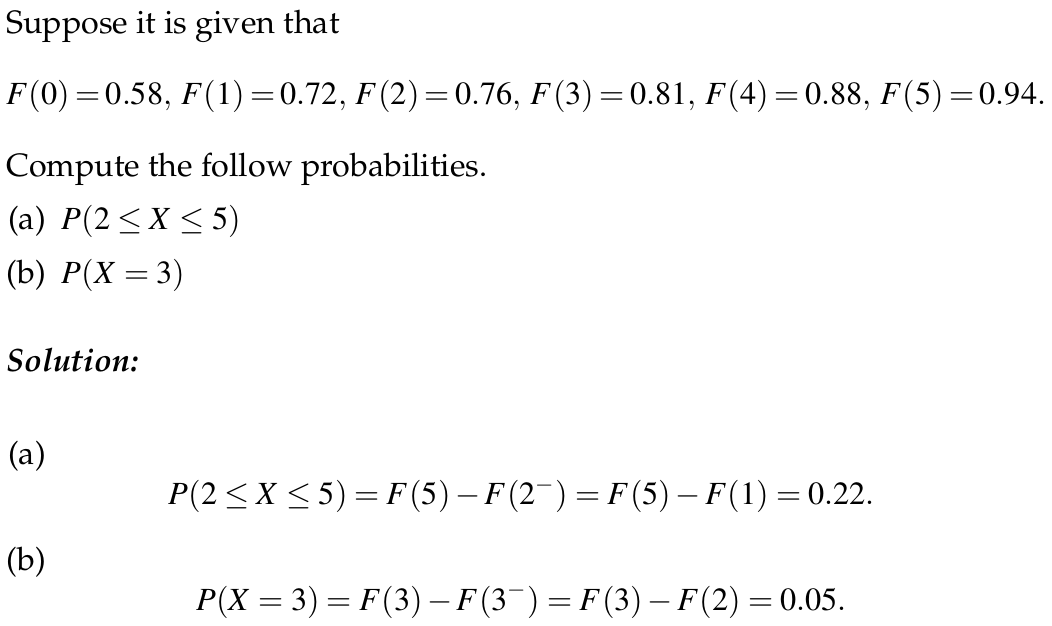
\includegraphics[scale=0.25]{pmf-find-p.png}
\noindent\rule{\columnwidth}{0.5pt}
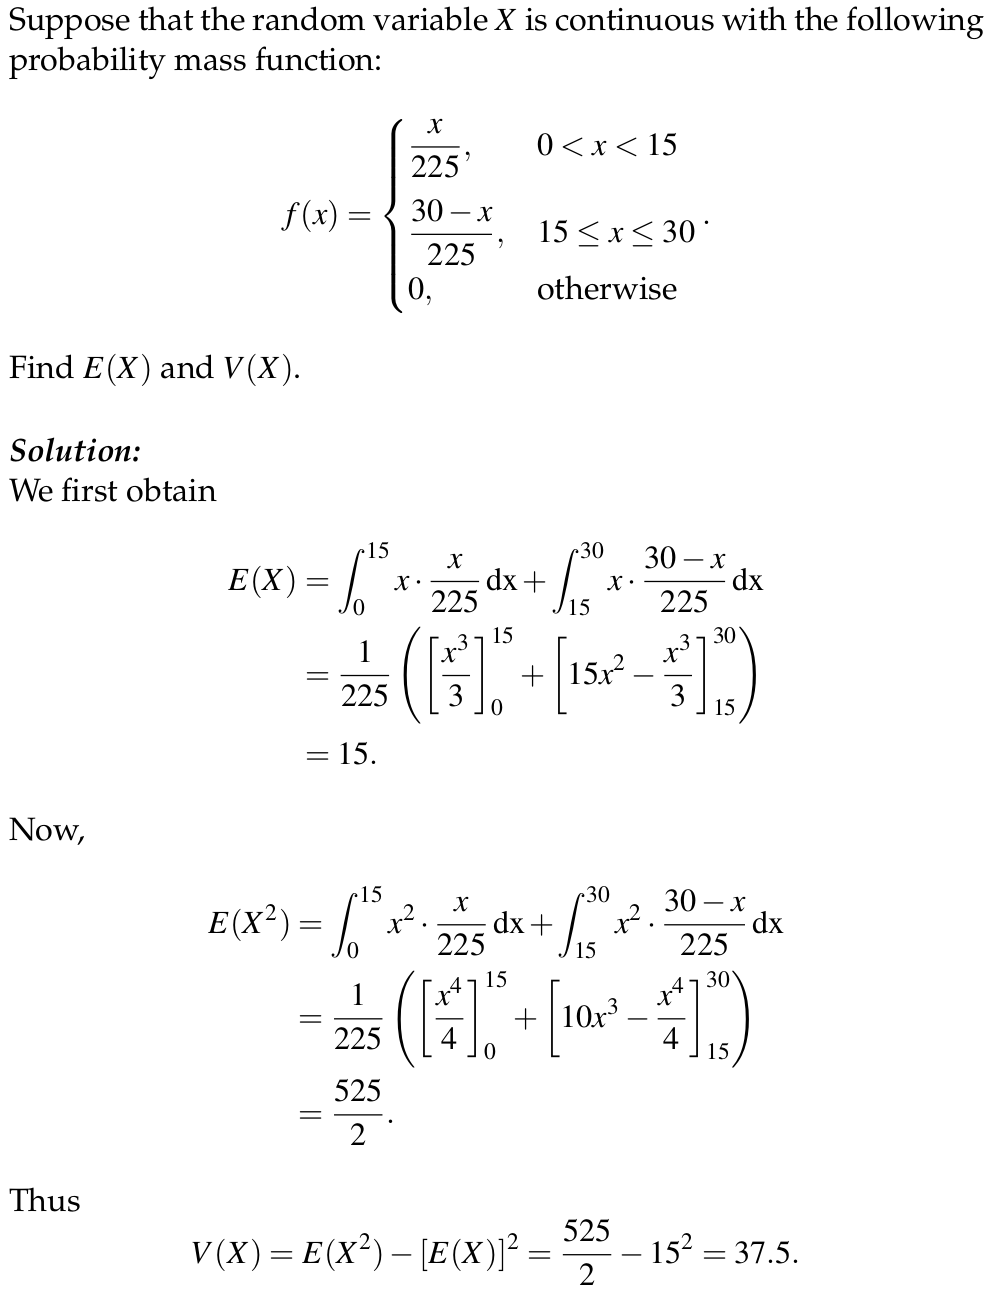
\includegraphics[scale=0.25]{pmf-e-v.png}
\noindent\rule{\columnwidth}{0.5pt}
%
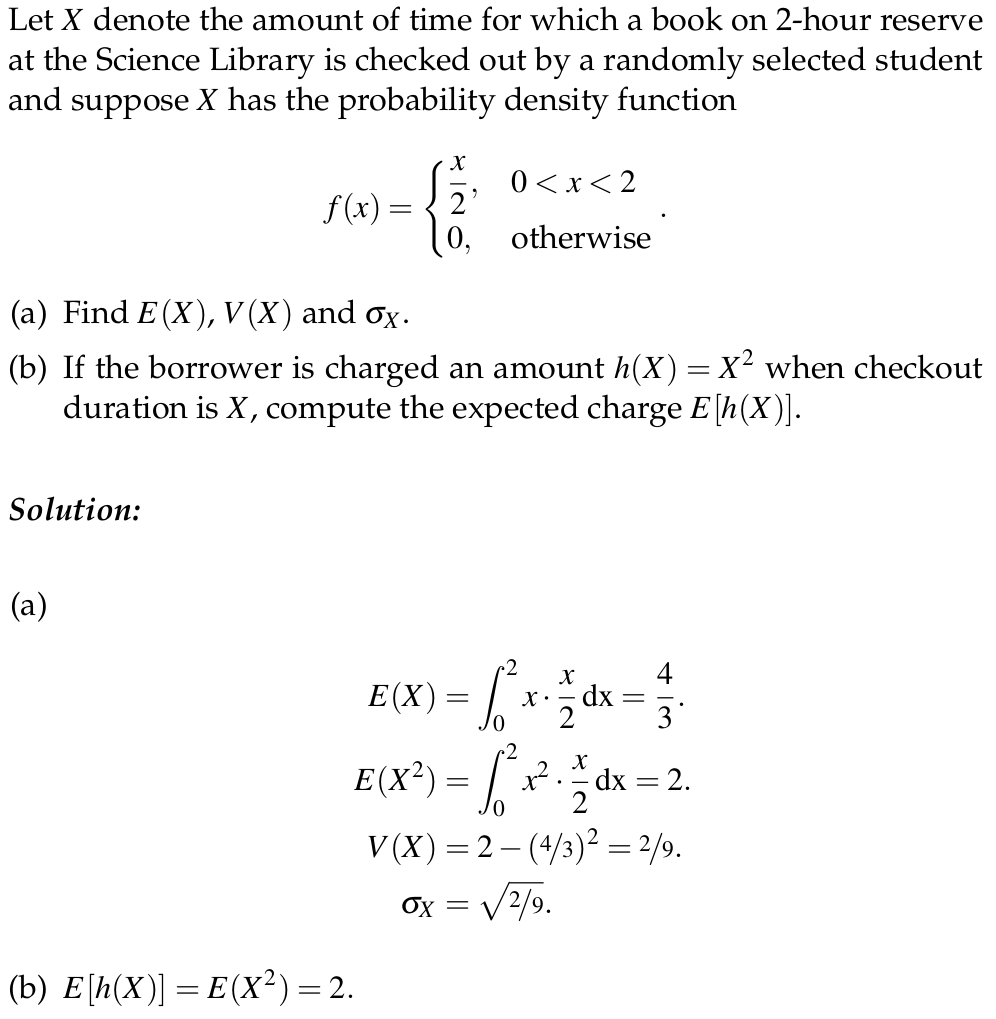
\includegraphics[scale=0.26]{pdf-find-e-v-sd.png}
\noindent\rule{\columnwidth}{0.5pt}
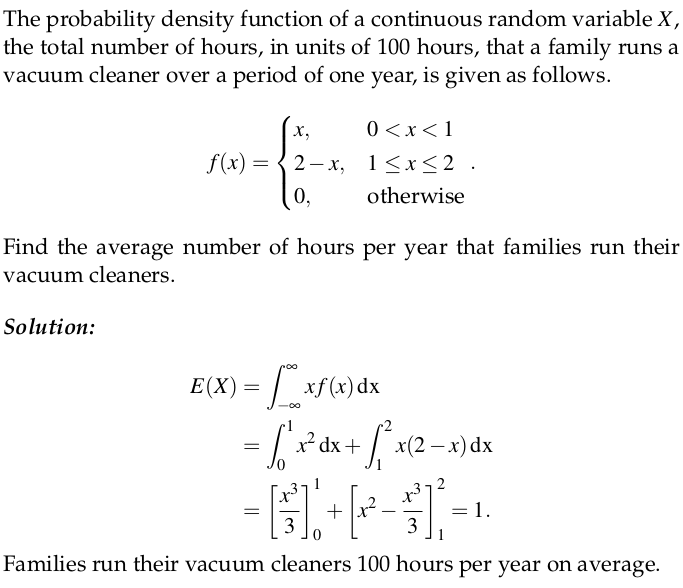
\includegraphics[scale=0.35]{pdf-find-e.png}
\noindent\rule{\columnwidth}{0.5pt}
%
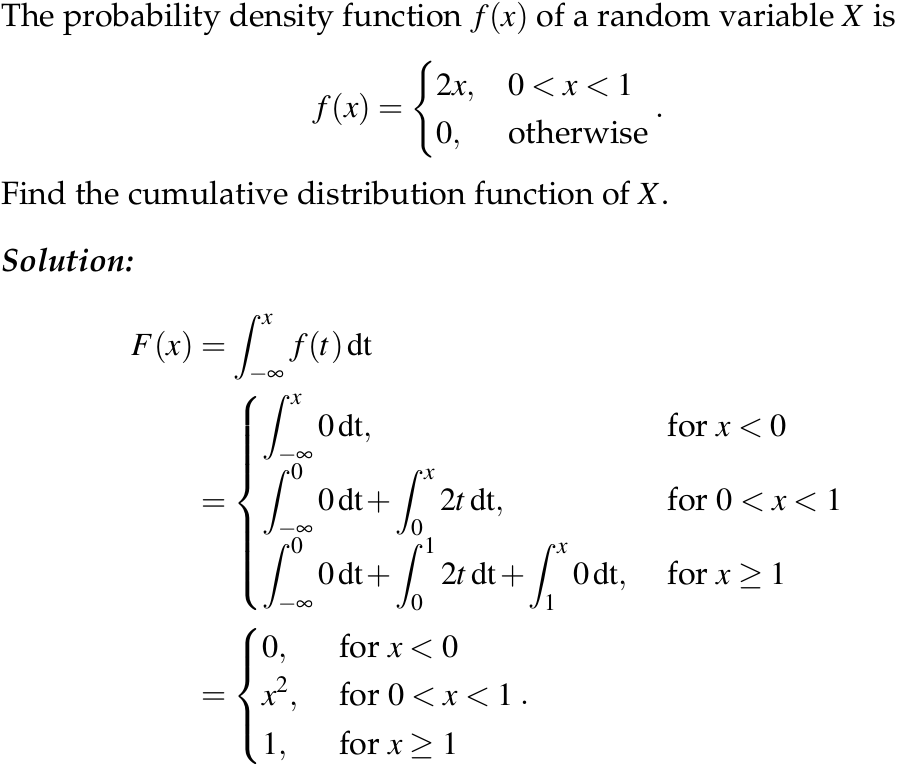
\includegraphics[scale=0.25]{pdf-find-cdf.png}
\noindent\rule{\columnwidth}{0.5pt}
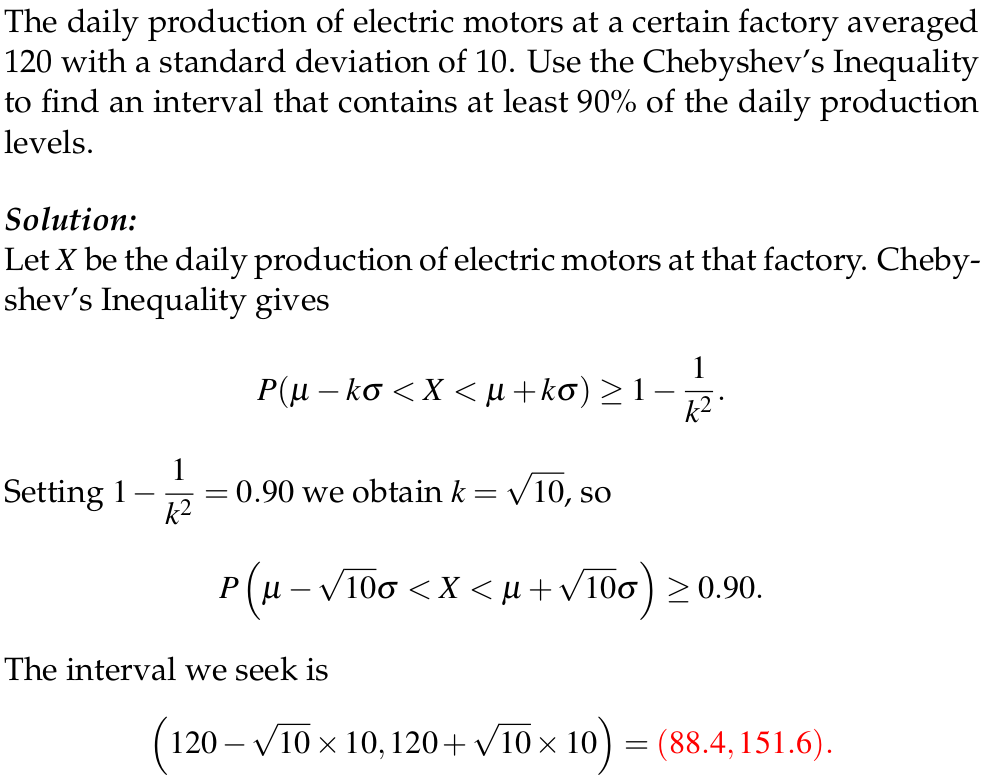
\includegraphics[scale=0.25]{chebyshev.png}
\noindent\rule{\columnwidth}{0.5pt}
%
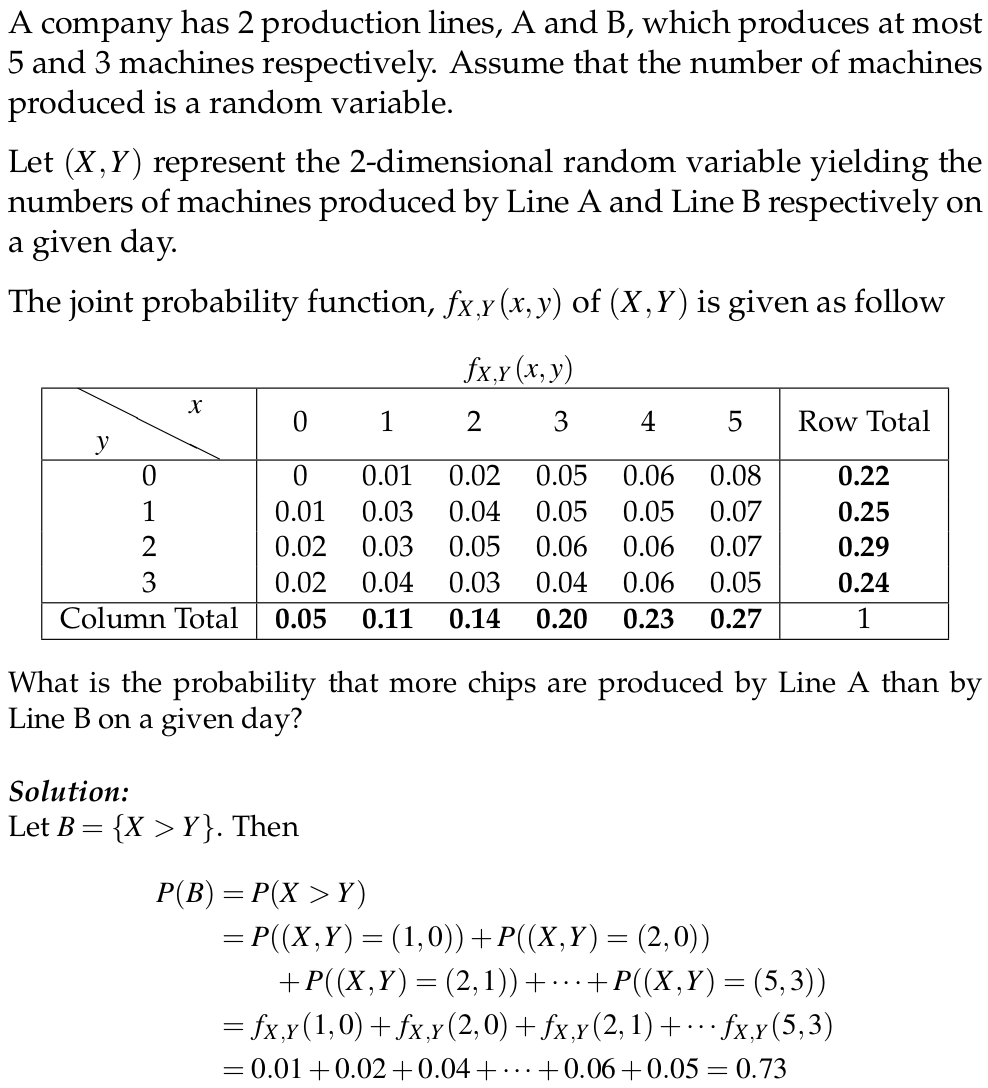
\includegraphics[scale=0.25]{jpmf-find-p.png}
\noindent\rule{\columnwidth}{0.5pt}
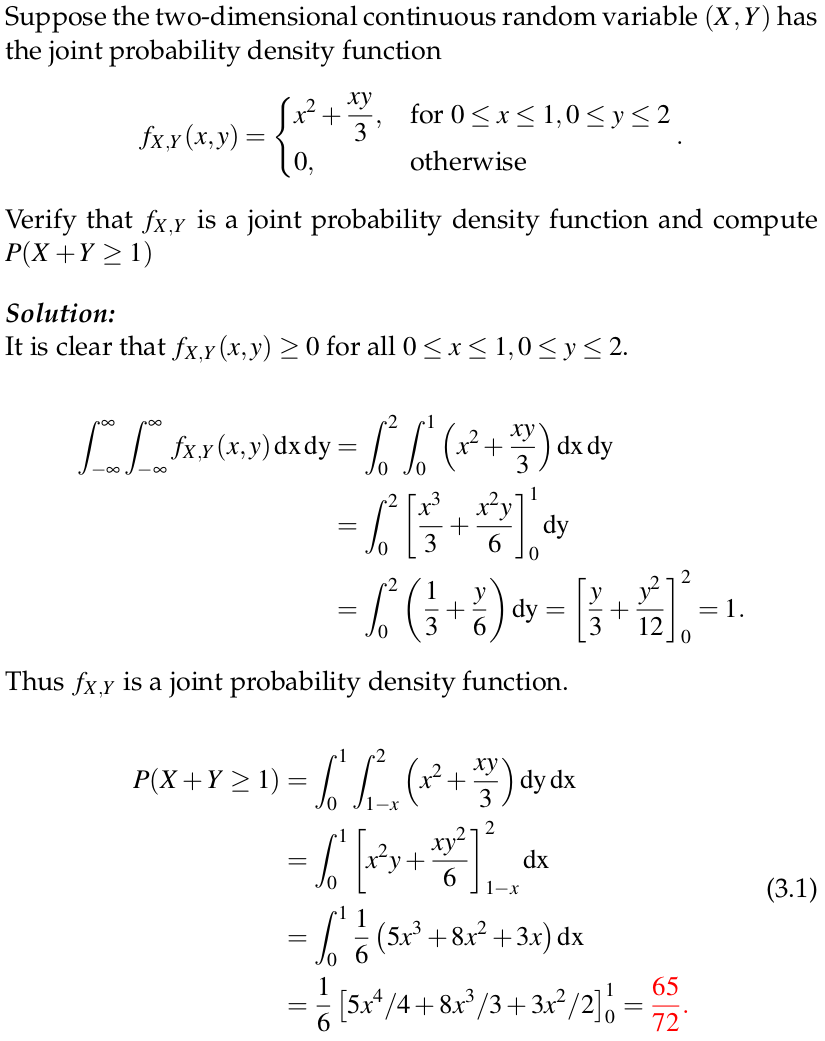
\includegraphics[scale=0.26]{jpdf-find-p.png}
\noindent\rule{\columnwidth}{0.5pt}

\end{multicols*}
\end{document}
